\usetikzlibrary {automata,positioning}
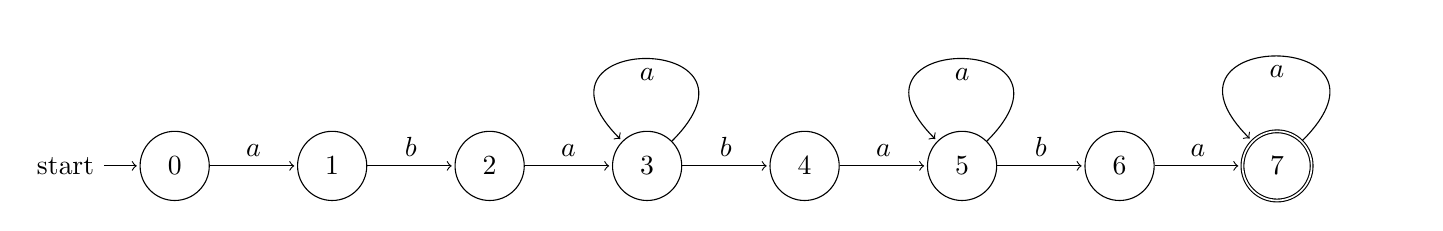
\begin{tikzpicture}[shorten >=1pt,node distance=2cm,on grid,auto]
	\node[initial,state] (0) {0};
	\node[state,right of=0] (1) {1};
	\node[state,right of=1] (2) {2};
	\node[state,right of=2] (3) {3};
	\node[state,right of=3] (4) {4};
	\node[state,right of=4] (5) {5};
	\node[state,right of=5] (6) {6};
	\node[accepting,state,right of=6] (7) {7};
	\path (0) edge[->] node {$a$} (1)
		 (1) edge[->] node {$b$} (2)
		 (2) edge[->] node {$a$} (3)
		 (3) edge[->] node {$b$} (4)
		 (4) edge[->] node {$a$} (5)
		 (5) edge[->] node {$b$} (6)
		 (6) edge[->] node {$a$} (7)
		 (3) edge[loop] node {$a$} (3)
		 (5) edge[loop] node {$a$} (5)
		 (7) edge[loop] node {$a$} (7);
\end{tikzpicture}
